\chapter{Boltzmann Inversion}

\hyperref[sec:bi]{Boltzmann inversion} provides a potential of mean force for a given degree of freedom. 
%
\begin{wrapfigure}{t}{7cm}
   \centering
   \includegraphics[width=7cm]{usage/fig/flow_boltzmann.eps}
   \caption{Flowchart deminstrating useful options of the tool.}
\end{wrapfigure}
%
It is mostly used for deriving {\em bonded} interactions from canonical sampling of a single molecule in vacuum, e.~g. for polymer coarse-graining, where it is difficult to separate bonded and non-bonded degrees of freedom~\cite{Tschoep:1998}. The non-bonded potentials can then be obtained by using iterative  methods or force matching.

The main tool which can be used to calculate histograms, cross-correlate coarse-grained variables, create exclusion lists, as well as prepare tabulated potentials for coarse-grained simulations is \prog{csg_boltzmann}.  It parses the whole trajectory and stores all information on bonded interactions in memory, which is useful for interactive analysis. For big systems, however, one can run out of memory. In this case \prog{csg_stat} can be used which, however, has a limited number of tasks it can perform.

Another useful tool is \prog{csg_map}. It can be used to convert an atomistic trajectory to a coarse-grained one, as it is discussed in sec.~\ref{sec:trajectory}.

To use \prog{csg_boltzmann} one has to first define a mapping scheme. This is outlined in~\sect{sec:mapping}. Once the mapping scheme is specified, it is possible to generate an exclusion list for the proper sampling of the atomistic resolution system. 

\section{Generating exclusion lists}
\label{sec:exclusions}
Exclusion lists are useful when sampling from a special reference system is needed, for example for polymer coarse-graining with a separation of bonded and non-bonded degrees of freedom.

To generate an exclusion list, an atomistic topology without exclusions and a mapping scheme have to be prepared first. Once the .tpr topology and .xml mapping files are ready, simply run
\begin{verbatim}
  csg_boltzmann --top topol.tpr --cg mapping.xml --excl exclusions.txt
\end{verbatim}
This will create a list of exclusions for all interactions that are not within a bonded interaction of the coarse-grained sub-bead. As an example, consider coarse-graining of a linear chain of three beads  which are only connected by bonds. In this case, \prog{csg_boltzmann} will create exclusions for all non-bonded interactions of atoms in the first bead with atoms of the 3rd bead as these would contribute only to the non-bonded interaction potential. Note that \prog{csg_boltzmann} will only create the exclusion list for the fist molecule in the topology.

To add the exclusions to the \gromacs topology of the molecule, either include the file specified by the --excl option into the .top file as follows
\begin{verbatim}
  [ exclusions ]
  #include "exclusions.txt"
\end{verbatim}
or copy and paste the content of that file to the exclusions section of the gromacs topology file.

\section{Statistical analysis}
For statistical analysis \prog{csg_boltzmann} provides an interactive mode. To enter the interactive mode, use the \progopt{--trj} option followed by the file name of the reference trajectory 
\begin{verbatim}
  csg_boltzmann --top topol.tpr --trj traj.trr --cg mapping.xml
\end{verbatim}
%
To get help on a specific command of the interactive mode, type
\begin{verbatim}
  help <command>
\end{verbatim}
for example
\begin{verbatim}
  help hist
  help hist set periodic
\end{verbatim}
%
Additionally, use the
\begin{verbatim}
  list
\end{verbatim}
command for a list of available interactions. Note again that \prog{csg_boltzmann} loads the whole trajectory and all information on bonded interactions into the memory. Hence, its main application should be single molecules. See the introduction of this chapter for the \prog{csg_stat} command.

If a specific interaction shall be used, it can be referred to by
\begin{verbatim}
  molecule:interaction-group:index
\end{verbatim}
Here, \texttt{molecule} is the molecule number in the whole topology, \texttt{interaction-group} is the name specified in the \texttt{<bond>} section of the mapping file, and \texttt{index} is the entry in the list of interactions. For example, \texttt{1:AA-bond:10} refers to the 10th bond named \texttt{AA-bond} in molecule 1. To specify a couple of interactions during analysis, either give the interactions separated by a space or use wildcards (e.g. \texttt{*:AA-bond*}).

To exit the interactive mode, use the command \texttt{q}. 

If analysis commands are to be read from a file, use the pipe or stdin redirects from the shell.
\begin{verbatim}
  cat commands | csg_boltzmann topol.top --trj traj.trr --cg mapping.xml
\end{verbatim}

\subsection{Distribution functions and tabulated potentials}
Distribution functions (tabulated potentials) can be created with the \textit{hist} (\textit{tab}) command.
For instance, to write out the distribution function for all interactions of group AA-bond (where AA-bond is the name specified in the mapping scheme) to the file AA.txt, type
\begin{verbatim}
  hist AA.txt *:AA-bond:*
\end{verbatim}
The command
\begin{verbatim}
  hist set
\end{verbatim}
prints a list of all parameters that can be changed for the histogram: the number \textit{n} of bins for the table, bounds \textit{min} and \textit{max} for table values, scaling and normalizing, a flag \textit{periodic} to ensure periodic values in the table and an \textit{auto} flag. If \textit{auto} is set to 1, bounds are calculated automatically, otherwise they can be specified by \textit{min} and \textit{max}. Larger values in the table might extend those bounds, specified by parameter \textit{extend}.

To directly write the Boltzmann-inverted potential, the \textit{tab} command can be used. Its usage and options are very similar to the \textit{hist} command. If tabulated potentials are written, special care should be taken to the parameters \textit{T} (temperature) and the \textit{scale}. The \textit{scale} enables volume normalization as given in \eq{eq:boltzmann_norm}. Possible values are \textit{no} (no scaling), \textit{bond} (normalize bonds) and \textit{angle} (normalize angles). To write out the tabulated potential for an angle potential at a temperature of 300K, for instance, type:
\begin{verbatim}
  tab set T 300
  tab set scale angle
  tab angle.pot *:angle:*
\end{verbatim}
The table is then written into the file \texttt{angle.pot} in the format \todo. An optional correlation analysis is described in the next section. After the file has been created by command \texttt{tab}, the potential is prepared for the coarse-grained run in chapter \ref{sec:usage:cgrun}.

\subsection{Correlation analysis}
The factorization of $P$ in \eq{eq:boltzmann_pmf} assumed uncorrelated quantities. \prog{csg_boltzmann} offers two ways to evaluate correlations of interactions. One option is to use the linear correlation coefficient (command \textit{cor}). However, this is not a good measure since \textit{cor} calculates the linear correlation only which might often lead to misleading results~\cite{Ruehle:2009.a} (An example are the two correlated random variables $X \sim U[-1,1]$ with uniform distribution, and $Y:=X^2$. A simple calculation shows $cov(X,Y)=0$ and therefore $cor=\frac{cov(X,Y)}{\sqrt{var(X)var(Y)}}=0$). A better way is to create 2D histograms. This can be done by specifying all values (e.g. bond length, angle, dihedral value) using the command \textit{vals}, e.g.:
\begin{verbatim}
  vals vals.txt 1:AA-bond:1 1:AAA-angle:A
\end{verbatim}
This will create a file which contains 3 columns, the first being the time, and the second and third being bond and angle, respectively. Columns 2 and 3 can either be used to generate the 2D histogram, or a simpler plot of column 3 over 2, whose density of points reflect the probability.

Two examples for 2D histograms are shown below: one for the propane molecule and one for hexane.

\begin{figure}[b]
\begin{minipage}{4cm}
  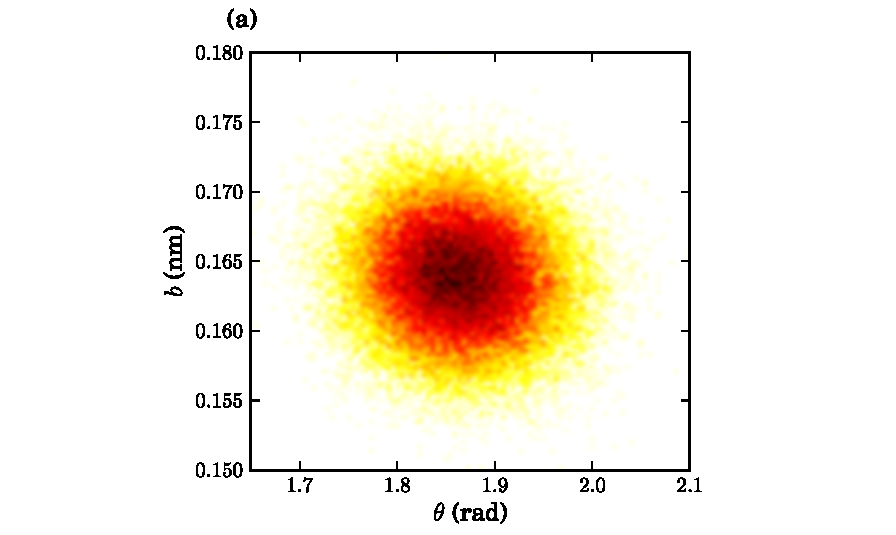
\includegraphics[height=3.1cm]{fig/propane_hist2d}
  \caption{propane histogram}
  \label{boltzmann:propane}
\end{minipage}
\hfill
\begin{minipage}{10cm}
  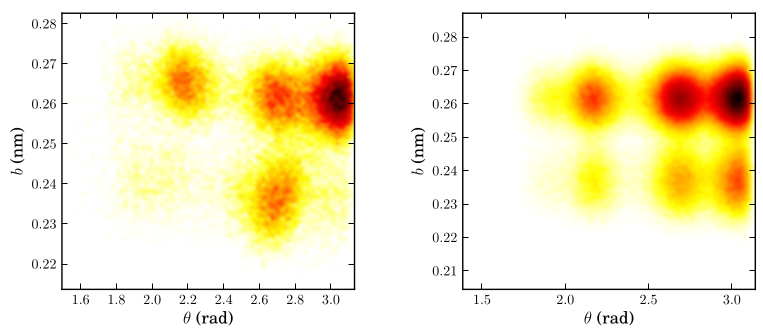
\includegraphics[height=4cm]{fig/hexane2}
  \caption{hexane histograms: before and after the coarse-grained run}
  \label{boltzmann:hexane}
\end{minipage}
\end{figure}

The two plots show the correlations between angle and bondlength for both molecules. In the case of propane, the two quantities are not correlated as shown by the centered distribution, while correlations exist in the case of hexane. Moreover, it is visible from the hexane plot that the partition of the correlations has changed slightly during coarse-graining.

The tabulated potentials created in this section can be further modified and prepared for the coarse-grained run: This includes fitting of a smooth functional form, extrapolation and clipping of poorly sampled regions. Further processing of the potential is decribed in chapter \ref{sec:usage:cgrun}.